\documentclass{beamer}
\usepackage{amsmath}
\usepackage{amsfonts}
\usepackage{amssymb}

%\usepackage{hyperref}

\usepackage{graphicx}
\usepackage{subfig}

\usepackage[english]{babel}
\usepackage[utf8]{inputenc}

\usepackage{multicol}
%\usepackage{natbib}%
\usepackage{units}

\usepackage{stmaryrd}
\usepackage{gensymb}
\usepackage{bibentry}
\usepackage{accents}

%\usepackage{booktabs}

\usepackage{tensor}
\usepackage[bbgreekl]{mathbbol}
\usepackage{bm}
\usepackage{ulem}

% FANCY TABLES
\usepackage{booktabs}
\usepackage{multirow}
\usepackage{threeparttable}

%\usetheme{Luebeck}
\usetheme{Madrid}
%\usetheme{CambridgeUS}
%\usetheme{Pittsburgh}
%\usetheme{default}
%\mode<presentation>

%FOR CAMBRIDGE US THEME -- red bullets/captions in itemize environment
\setbeamercolor{item projected}{bg=black}
\setbeamertemplate{enumerate items}[default]
\setbeamertemplate{navigation symbols}{}
\setbeamercovered{transparent}

\setbeamercolor*{enumerate item}{fg=black}
\setbeamercolor*{enumerate subitem}{fg=black}
\setbeamercolor*{enumerate subsubitem}{fg=black}

\setbeamercolor{block title}{fg=black}
\setbeamercolor{caption name}{fg=black}

\title[Spektrálne metódy]{Spektrálne kolokačné metódy a vlastnéčísla Laplaceovho operátora}
\author[Veronika Bozděchová, Jiří Púček, Marek Mikloš] {Veronika Bozděchová, Jiří Púček, Marek Mikloš \\ }
\institute[Charles University]{Charles University, Czech Republic}
\date{}




\let\newblock\relax

\newcommand{\smallbibentry}[1]{{\tiny \bibentry{#1}}}

% \AtBeginSection[]
% {
%   \begin{frame}
% %    \frametitle{Outline}
%     \tableofcontents[currentsection]
%   \end{frame}
% }

\begin{document}

\begin{frame}
\titlepage
\bibliographystyle{plain}
\nobibliography{vit-prusa}
\end{frame}

% \begin{frame}
%   \frametitle{Outline}
%   \tableofcontents
% \end{frame}

\section*{Úvod}
\label{sec:1}


\begin{frame}
 \frametitle{Úvod}

'Najprimitívnejší model pre vychýlenie dosiek je daný rovnicou'
\begin{equation}
\label{eq:1}
\frac{\partial ^2{u}}{\partial {t^{2}}}-K^{2}\Delta{u}=0,
\end{equation}
"kde $u$ je vychýlenie dané ako zobrazenie $u:(t,\vec{x}) \in \mathbb{R} \times \mathbb{R}^{2} \mapsto \mathbb{R}$"
"Pre stojaté vlnenie má riešenie \ref{eq:1} tvar:"
\begin{equation}
\label{eq:2}
-\Delta{\widehat{u}}=\frac{\omega^{2}}{K^{2}}\widehat{u}
\end{equation}
"Ak označíme $L=_{def}-\Delta$ a $\lambda=_{def}\frac{\omega^{2}}{K^{2}}$ z \ref{eq:2} dostaneme:"
\begin{equation}
\label{eq:3}
-L{\widehat{u}}=\lambda\widehat{u}
\end{equation}
"Z čoho dostaneme po dosadení vhodných okrajových podmienok úlohu pre nájdenie vlastných vektorov lineárneho operátora."

\end{frame}

\section*{Pokračovanie}
\label{sec:P}

\begin{frame}
    "Chceme nájsť vlastné vektory a vlastné čísla Laplaceovho operátora v $\Omega \subset \mathbb{R}^{2}$ s nulovou Dirichletovou podmienkou. Chceme teda riešiť:"

    \begin{subeqations}
    \label{eq:4}
    \begin{equation}
    \label{eq:5}
    -\Delta{\widehat{u}}=\lambda\widehat{u}
    \end{equation}

    \begin{equation}
    \label{eq:6}
    \widehat{u}|_{\partial{\Omega}}=0
    \end{equation}

    \end{subeqations}




    Hodnoty \widehat{u} v interpolačných $[x_{i},y_{k}]$ bodoch označíme ako $\widehat{u}_{i,k}$, dostávame:

    \begin{equation}
    \label{eq:6}
    \widehat{u}_{i,k}=_{def}(\widehat{u}_{x})_{i,k}=_{def}\widehat{u}(x_i,y_k).
    \end{equation}

    Aproximácie parciálnych derivácií podľa x a y budú označené ako $(\widehat{u}_{x})_{i,k}$ a $(\widehat{u}_{y})_{i,k}$. Teda

<<<<<<< HEAD


    \begin{subequations}
    \label{eq:7}
    \begin{equation}
    \label{eq:8}
    (\widehat{u}_{x})_{i,k}=_{def}\frac{\partial \widehat{u} }{\partial x}(x,y)\mid_{x=x_i,y=y_k}
    \end{equation}
    \begin{equation}
    \label{eq:9}
    (\widehat{u}_{y})_{i,k}=_{def}\frac{\partial \widehat{u} }{\partial y}(x,y)\mid_{x=x_i,y=y_k}
    \end{equation}
    \end{subequations}
\end{frame}


\section*{Vibrace destičky}
\label{sec:desticka}

\begin{frame}
  \frametitle{Výpočet v Matlabu a porovnání s Mathematicou}
  V následujích výpočtech jsme vždy uvažovali obdélník $2 \times 3$, s čímž nám vyšla následující vlastní čísla:

  \begin{array}
 \text{Matlab} & 3.56402 & 6.85389 & 10.9662 & 12.337 &
   14.2561 & 19.7392 & 20.0134 & 23.3031 & 26.593 &
   27.4156 & 29.883 & 32.0761 & 37.2852 & 39.7525 &
   40.5689 & 41.9457 \\
 \text{Mathematica} & 3.56403 & 6.85392 & 10.9665 &
   12.3373 & 14.2564 & 19.7397 & 20.0149 & 23.3061 &
   26.596 & 27.4174 & 29.8888 & 32.0794 & 37.2913 &
   39.7571 & 40.591 & 41.963 \\
  \end{array}
  

=======
\end{frame}
	\section*{Matlab kód}
\label{sec:xxxx}
\begin{frame}[fragile]
	\frametitle{Matlab kód}
	{\tiny
		Zadefinujeme jednotlivé konstanty a vektory, se kterými pracujeme (speciálně pro jeden pevný konec máme $a_4=\frac{F}{EIzz}=\frac{g\rho d a^2}{EIzz}$).
		\begin{verbatim*}
			g=9.81;rho=650;d=10;x=[-d/2,d/2];a=0.25;a1=0;a2=0;a3=0;a4=0;
			E=10^5;Izz=1;n=20;
		\end{verbatim*}
		Dále si vybereme funkci $f(x)$, která nám udává hustotu působící síly na jednotku délky. Tato funkce nám dává pravou stranu naší obyčejné diferenciální rovnice.
		\begin{verbatim*}
			f=@(x) -g*rho*a^2*1.^(x);
			L=E*Izz*diffmat([n n+4],4,x);
		\end{verbatim*}
		Pro případ dvou případně jednoho pevného konce volíme dané okrajové podmínky. V textu níže můžeme vidět příslušné rovnice příslušné okrajovým podmínkám pro jeden pevný konec (pro případ dvou pevných konců $T_1=T_3$,$T_2=T_4$ s tím, že hranice je nyní $+\frac{d}{2}$ místo $-\frac{d}{2}$).
		\begin{verbatim*}
			T1=diffrow(n+4,0,-d/2,x);T3=diffrow(n+4,1,-d/2,x);T2=diffrow(n+4,2,d/2,x);T4=diffrow(n+4,3,d/2,x);
		\end{verbatim*}
		Sestavíme naši maticovou soustavu a vyřešíme ji.
		\begin{verbatim*}
			A=[L;T1;T2;T3;T4];
			rhs=[gridsample(f,n);a1;a2;a3;a4];
			u=A\rhs;
		\end{verbatim*}
	}
\end{frame}

\begin{frame}
	\frametitle{Porovnání Mathematica x Matlab}
	\begin{minipage}{\textwidth}
		\begin{minipage}[b]{0.5\textwidth}
			\centering
			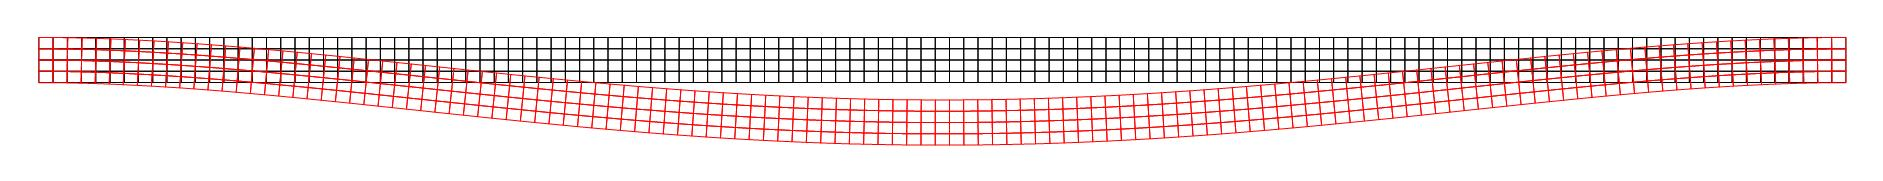
\includegraphics[width=1\textwidth]{1}
			\captionof*{figure}{\textbf{Obrázek 1.} Mathematica (pevné konce)}
		\end{minipage}
		\begin{minipage}[b]{0.5\textwidth}
			\centering
			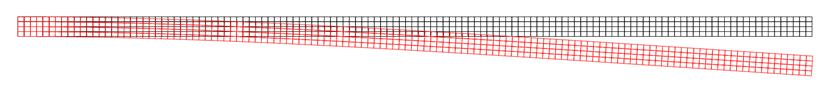
\includegraphics[width=1\textwidth]{2}
			\captionof*{figure}{\textbf{Obrázek 2.} Mathematica (pevný konec)}
		\end{minipage}
		\hfill
	\end{minipage}
	\begin{minipage}{\textwidth}
		\begin{minipage}[b]{0.5\textwidth}
			\centering
			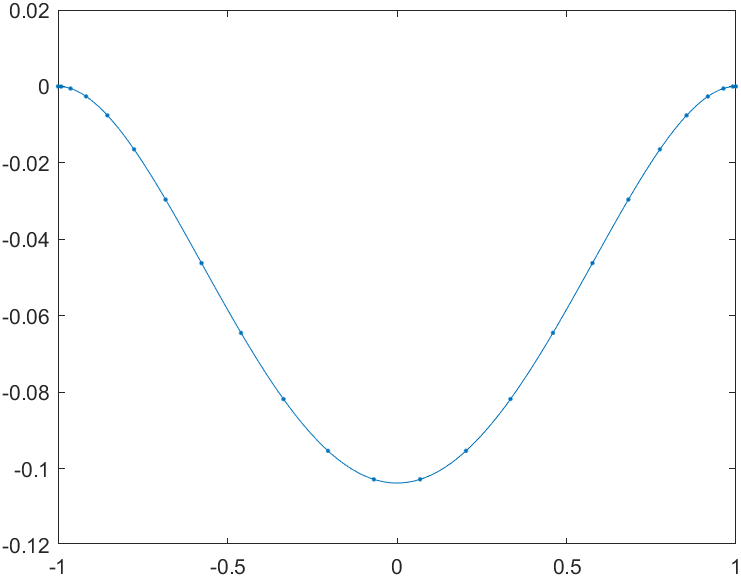
\includegraphics[width=0.7\textwidth]{untitled1}
			\captionof*{figure}{\textbf{Obrázek 3.} Matlab (pevné konce)}
		\end{minipage}
		\begin{minipage}[b]{0.5\textwidth}
			\centering
			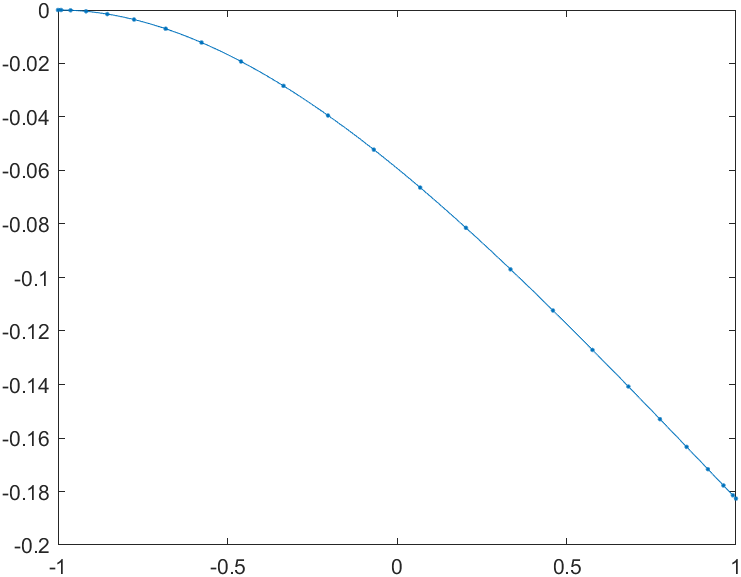
\includegraphics[width=0.7\textwidth]{untitled2}
			\captionof*{figure}{\textbf{Obrázek 4.} Matlab (pevný konec)}
		\end{minipage}
		\hfill
	\end{minipage}
>>>>>>> 5d3b185b0a81359fcf1384b4364b0b263ba0b5f3
\end{frame}

\begin{frame}
  \frametitle{Matlab vs Mathematica}
  \begin{figure}[ht]
    \centering
    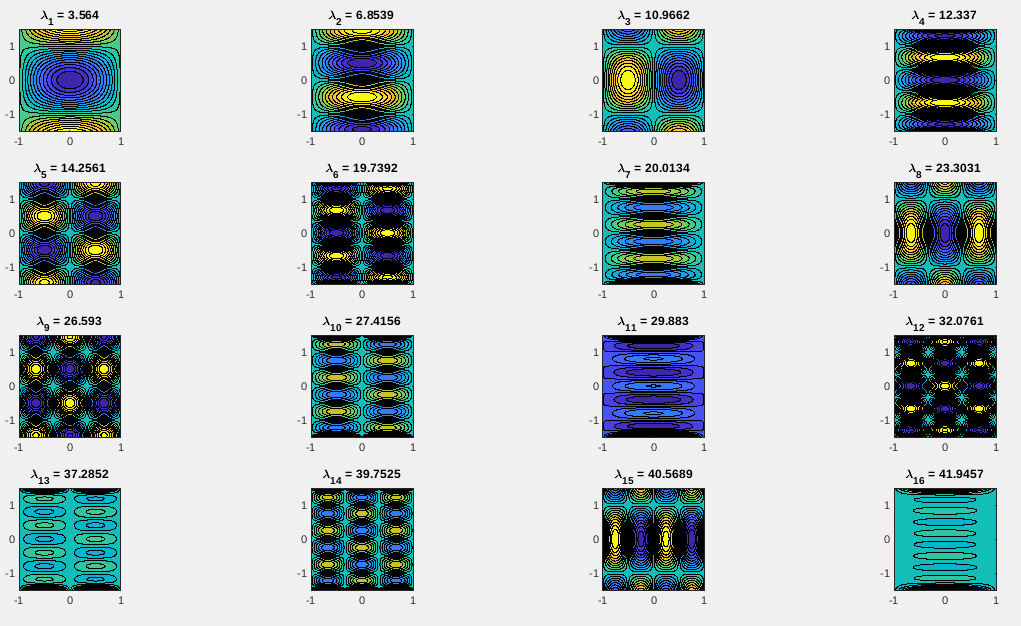
\includegraphics{barevne.png}
    \caption{\label{fig:label} Matlab s barvami}
  \end{figure}

\end{frame} 

\begin{frame}
  \frametitle{Matlab vs Mathematica}
  \begin{figure}
    \centering
    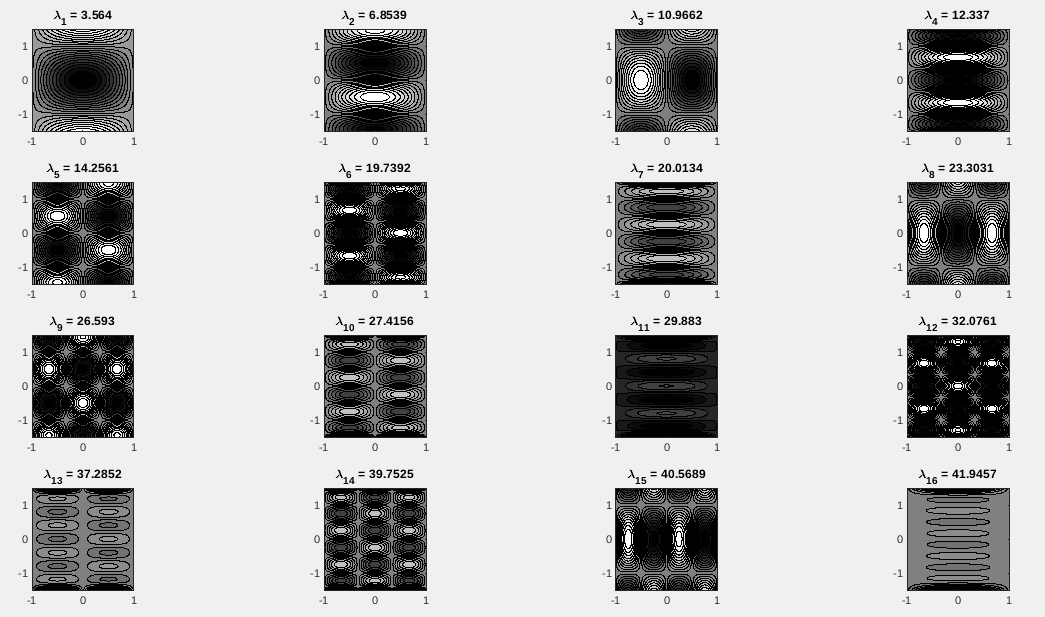
\includegraphics{sede1.png}
    \caption{V monochronních barvách}
  \end{figure}
\end{frame}

\begin{frame}
  \frametitle{Matlab vs Mathematica}
  \begin{figure}[h!]
    \centering
    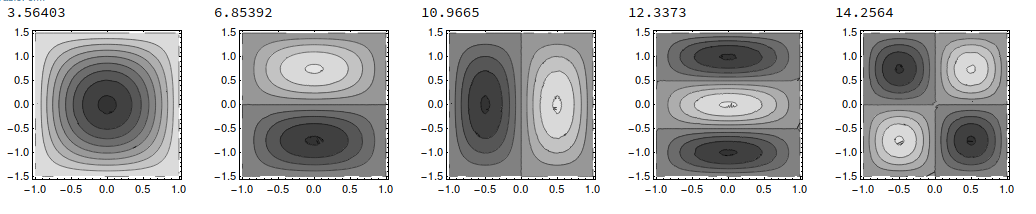
\includegraphics[width = 0.75\textwidth]{mathematica1.png}
    \caption{Mathematical plot}
  \end{figure}
  
  \begin{figure}[h!]
    \centering
    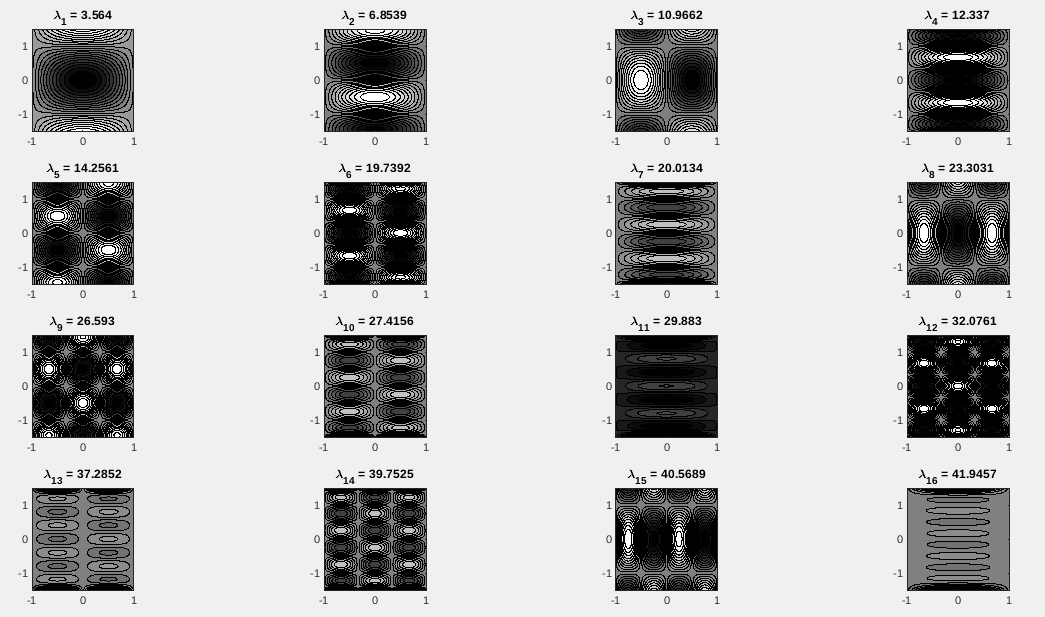
\includegraphics[width = 0.75\textwidth]{sede1.png}
    \caption{Matlab plot}
  \end{figure}
\end{frame}


\end{document}
<<<<<<< HEAD

%                 
%
%
%
% DOCUMENT ENDS HERE
%
%
%
%
=======
>>>>>>> 5d3b185b0a81359fcf1384b4364b0b263ba0b5f3
